\documentclass[a4paper,11pt]{article}
\usepackage[utf8]{inputenc}
\usepackage[T1]{fontenc}
\usepackage[french]{babel}
\usepackage{textcomp}
\usepackage{listings}
\usepackage{pdfpages}
\usepackage{array}

\title{PROJET\\ UE Méthodes de ranking et recommandations\\ 
		Sujet 5 : Simulation d'un Google Bombing}
\author{Maxime Gonthier - Laureline Martin}

\begin{document}

\pagenumbering{gobble}\clearpage
	\pagenumbering{gobble}\clearpage
	\maketitle
	\newpage\clearpage\pagenumbering{arabic}

\newpage
\tableofcontents

\newpage
\section{Introduction}
	Le but de ce projet est de simuler, d'évaluer et de proposer la méthode la plus efficae pour un Google Bombing. Il s'agit d'une technique d'attaque sur le graphe du web afin d'augmenter la pertinence d'une page cible. Pour cela, plusieurs attaquants créent des pages et y insèrent des liens vers une page cible à attaquer. Plusieurs structures de pages attaquantes sont possibles :
	\begin{itemize}
		\item seul
		\item complet
		\item anneau
		\item arbre
	\end{itemize}
	Nous allons tester ces différentes structures sur des pages de pertinences différentes et déterminer quelle est la structures la plus avantageuse pour obtenir la pertinence la plus forte possible.

\section{Manuel utilisateur}
	Notre application se lance grâce à la commande \texttt{make all} suivie de fichier ".txt" à modifier.
	\texttt{make clean} pour nettoyer et \texttt{make compil} pour simplement compiler.\\
	Apres le make all voila ce qui s'affiche : \\
	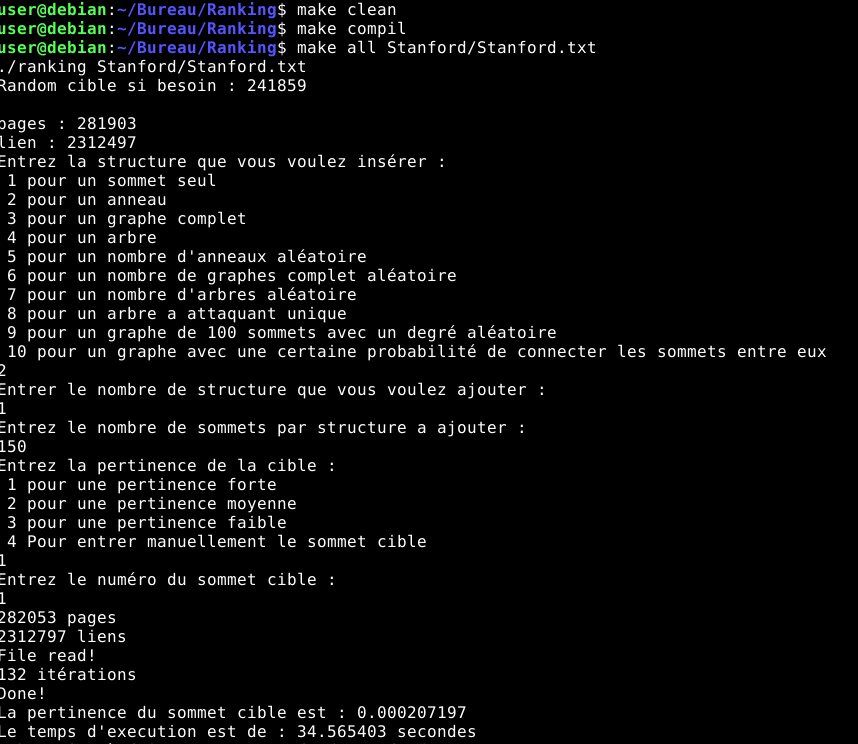
\includegraphics[scale = 0.5]{Captures/manuel.png}\\
	Dans un premier temps l'utilisateur choisis la structure qu'il veut ajouter au graphe du web.
	Il y a des structures simples (arbre, anneau, graphe complet sommet seuls), des structures moins conventionelles (arbre a attaquant unique, un arbre ou seul le sommet racine pointe vers la cible).
	On peut aussi ajouter un nombre de structures aléatoires (avec une limitation de 100 sommets). On peut également insérer un graphe de degré aléatoire ou un graphe dont le degré est une probabilité.
	Ensuite l'utilisateur va entrer le nombre de structures qu'il veut, cela ne s'applique pas pour les structures numéro 5,6 et 7. 
	Ensuite on entre le nombre de sommets de la ou les structures à ajouter. 
	Puis on entre le sommet cible. Le numéro du sommet cible est demandé une seconde fois pour savoir quel sommet sera donné en résultats.
	Enfin le programme affiche le nombre de pages/liens, le temps d'éxecution et la pertinence du sommet cible.\\
	

\section{Plan}
	Dans un premier temps nous allons effectué des tests simples en utilisant quatre type de structures différentes ainsi que trois cibles de pertinences différentes.
	Nous en déduirons des hypothèses sur l'eficacité de chaque structure et l'impact de la pertinence de la cible sur cette même efficacité.
	Dans un second temps nous étudierons l'impact sur la pertinence de graphes générés en nombre aléatoire pour étudier qu'elle structure est globalement la plus efficace.
	Puis nous testerons la meme choses avec cette fois ci un graphe dont les arcs le reliant a lui meme sont générées aléatoirement.
	Enfin nous ferons varier le nombre de sommets du graphe ataquant pour en déduire son efficacité et nous conclurons.
	
\section{I.	Tests initiaux et hypothèses}
	L'algorithme power calculant les pertinences est contenu dans le fichier $ranking.c$. Il n'est pas détaillé dans ce rapport mais le fichier est commenté.
	On considère ici le graphe du web Stanford.txt. Ce graphe est modifié par l'ajout de sommets et d'arcs afin d'augmenter la valeur d'un sommet ciblé.\\
	On considère que :\\
	\begin{itemize}
		\item Les sommets représentent les pages du web.
		\item Les arcs représentent les liens dirigeant vers d'autres pages.
		\item Les valeurs des sommets représentent les pertinences calculés par l'algorithme pagerank.
		\item Le sommet cible représente la page dont on souhaite augmenter la pertinence.
		\item 100 sommets sont ajoutés pour chaque test.
	\end{itemize}
	\subsection{Explications du code}
	Le code est contenu dans les fonctions $ajoutanneau$, $ajoutsommetseul$, $ajoutcomplet$ et $ajoutarbre$. Ces fonctions vont créer des structures à la fin du fichier. Ils
	prennent en argument $nbajout$ : le nombre de sommets par structures, $nom$ : le nom du fichier contenant le graphe du web, $nbpages$ et $nbliens$ : le nombre de pages et de lien du graphe du web, $perticible$ la cible à attaquer et $nbstructure$ : le nombre de structures à ajouter.\\
	Décrivons $ajoutanneau$ : 
	\begin{lstlisting}
FILE *g = fopen(nom,"a");
for (int y = 0; y < nbstructure; y++) {
	for (i = 1; i < nbajout; i++) {
		fprintf(g, "%d %d %d 0.500000 %d 0.500000\n", 
			nbpages+i+(y*nbajout), degre, 
			nbpages+i+1+(y*nbajout), cible);
	}
	//ecriture du dernier sommet qui se relie au 
	//premier sommet de l'anneau
	fprintf(g, "%d %d %d 0.500000 %d 0.500000\n", 
		nbpages+i+(y*nbajout), degre, 
		nbpages+1+(y*nbajout), cible);
}
	\end{lstlisting}
	Ici $y$ et $i$ vont incrémenter respectivement le nombre de structures et le sommet suivant à ecrire. $i$ commence à 1 pour écrire le numéro de page suivant le dernier numéro de page du graphe. 
	Ensuite on écris le nouveau nombre de pages et de lien du graphe de cette mainière :
	\begin{lstlisting}
	fprintf(h, "%d %d", nbpages+(nbajout*nbstructure),
	 nbliens+(nbajout*nbstructure)*2);
	\end{lstlisting}
	Décrivons $ajoutcomplet$ :
	\begin{lstlisting}
for (int y = 0; y < nbstructure; y++) {
	for (i = 1; i < nbajout + 1; i++) {
		fprintf(g, "%d %d", nbpages+i+(y*nbajout), degre);
		for(j = 1; j < nbajout + 1; j++){
			if (nbpages+j == nbpages+i) {}
			else {
				fprintf(g, " %d %f", 
					nbpages+j+(y*nbajout), x);}
		}
		fprintf(g, " %d %f\n", cible, x);
}	
	\end{lstlisting}
	Ici le premier printf écris le numéro de la page courante et son degré. Le second printf va écrire les liens entre cette page et toutes les autres pages du graphe complet. Le if sert à vérifier que l'on écrit pas un lien de la page vers elle-même.\\
	Décrivons $ajoutarbre$ :
	\begin{lstlisting}
for (int y = 0; y < nbstructure; y++) {
	// Initialisation du sommet racine
	racine = nbpages + 1+(y*nbajout);
	fprintf(g, "%d %d %d 1.000000\n", racine, 1, cible);
	// Sommets 2 a 2 (arbre binaire) et on pointe 
	//vers le sommet pere 
	// lui meme calcule par sa distance a la racine	
	for (i = 1; i < nbajout - 1; i+=2) {
		fprintf(g, "%d %d %d 0.500000 %d 0.500000\n", 
			racine+i, degre, racine + compteur, cible);	
		fprintf(g, "%d %d %d 0.500000 %d 0.500000\n", 
			racine+i+1, degre, racine + compteur, cible);	
		compteur++;
	}
	// Le dernier sommet dans le cas d'un nombre 
	//PAIR de sommets 
	// a entrer (pair car le sommet racine est deja 
	//ecris hors de la boucle)
	if (nbajout%2 == 0){ 
		fprintf(g, "%d %d %d 0.500000 %d 0.500000\n", 
			racine+i, degre, racine + compteur, cible);
	}
	//on reinitialise le compteur car on va commencer
	//un nouvel arbre
	compteur = 0;
}
	\end{lstlisting}
	Ici $racine$ représente le sommet racine et va servir à ecrire les pages suivantes. Les pages sont écrites deux à deux et calculé avec leurs distance par rapport à $racine$. Elle sont écrite deux à deux car on écrit les deux fils d'un sommet père à chaque itérations. $compteur$ est utilisé dans le cas de la création de plusieurs arbres.

	\subsection{Résultats des tests initiaux}
		\subsubsection{Stanford.txt sans modification}
			281903 pages\\
			2312497 liens\\
			132 itérations\\
			27.627466 secondes\\
			\\
			Voici les pertinences de base des trois sommets étudiés :\\
			Pertinence forte : Page 280545 - 9.96199e-05\\
			Pertinence moyenne : Page 281466 - 7.53954e-06\\
			Pertinence faible : Page 281574 - 6.05222e-07\\
			\\
		\subsubsection{Résultats}
			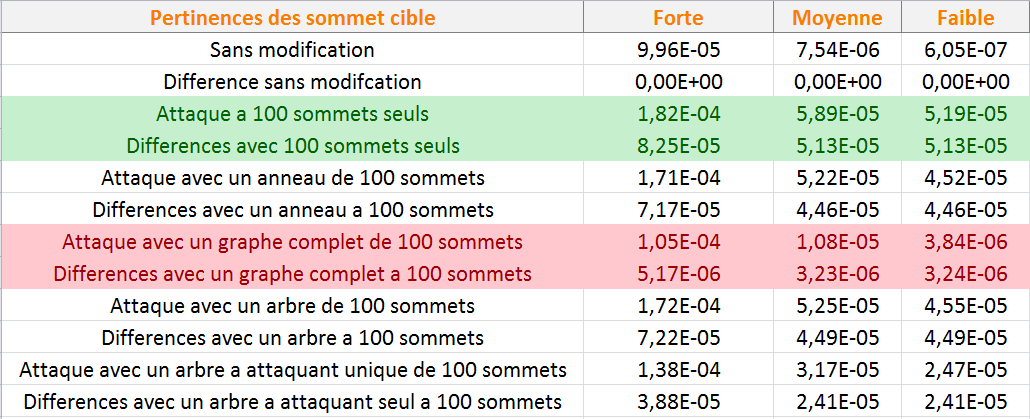
\includegraphics[scale = 0.5]{Captures/ranking1.PNG}

	\subsection{Conclusion des tests initiaux}
		Cinq structures différentes sont ajoutées : des sommets seuls, un graphe complet, un anneau, un arbre et un arbre a attaquant unique. L'arbre a attaquant unique est un arbre dont seul le sommet racin est relié 
		à la cible. L'objectif de cette structure est de minimiser le nombre de sommets reliées a la cible pour ainsi minimiser les chances de se faire repérer lors de l'attaque.\\
		On observe pour chaque cible que la structure la plus efficace est le sommet seul, suivis de l'arbe, de l'anneau, de l'arbre a attaquant unique et enfin du graphe complet.\\
		La raison de cette ordre serait que pour des sommets seuls, la probabilité de pointer sur la cible est de 1/1 alors qu'elle est de 1/n pour un graphe complet
		avec n le nombre de sommets. Ainsi la probabilité est dilué et donc la cible en sera moins modifié.\\
		On observe que pour chaque structure la différence de modification de la pertinence est presque identique entre les cibles faibles et moyennes.
		Ainsi on peut en déduire que modifier la pertinence d'une cible à e-06 ou e-07 est de même difficulté.\\		
		Pour le sommet sommet seul on observe que la modification de pertinence (la différence) pour une cible forte, moyenne ou faible sont respectivements
		8.25e-05, 5.13e-05 et 5.13e-05. Ainsi on peut en déduire que modifier la pertinence est plus significatif quand la cible est déjà forte.
			
		\subsubsection{Hypothèses}
			On suppose que les structures les plus efficaces sont les sommets seuls et les arbres. On suppose que changer la pertinence d'une cible devient 
			plus difficile à partir d'une cible de pertinence Xe-05 et que c'est assez identique pour les cibles de pertinences Xe-06 et Xe-07.


\section{II.	Tests avec un nombre de graphes générés aléatoirement}
	Nous allons désormais insérer des graphes générés aléatoirement. Ce qui est aléatoire n'est pas la structure des graphes mais le nombre de garphes générés.\\
	L'objectif de cette démarche est de déterminer quel structure est la plus efficace globalement.\\
	C'est a dire quelle structure influe le plus sur la pertinence quelle que soit la situation.\\
	De plus les resultats nous aiderons aussi a determiner l'impact qu'a une certaine structure sur la cible de manière plus générale 
	que dans les cas prédéfinis de la partie précedente.
	Le nombre de sommet des graphes ajoutées est fixé a 100.
	La cible est également fixé ainsi que la structure des graphes ajoutées.
	On va par exemple insérez 5 graphes complet de nombre de sommet respectivement : 25, 10, 5, 6 et 4. Tous reliées au sommet cible.
	Dans un premier temps nous allons expliquer le code derrière cette démarche puis nous analyserons les résultats.

	\subsection{Explication du code}
		Tous est dans le fichier $ajoutsommetsattanquants.c$. Les fonctions utilisées sont $ajoutanneaualeatoire$, $ajoutcompletaleatoire$
		et $ajoutarbrealeatoire$. Ces fonctions reprennent en partie le code des trois fonctions presque eponyme décrite précedemment.
		Regardons ce qui a changé. 
		\begin{lstlisting}
while(nbsommetrestant > 0) {
	nbajout = rand()%(100-nouveausommets);
	if (nbajout <= 3) { nbajout = 3; }
	nbsommetrestant -= nbajout;
		\end{lstlisting}
		$nbajout$ représente le nombre de sommet que l'on va ajouter dans la première structure créer. Il choisis donc un nombre 
		aléatoire entre 0 et 100 car le nombre de sommet total est limité a 100. Si le nombre choisis est inférieur a 3 on le fixe a 3 car créer
		des anneau ou des graphes complets de tailles inférieure a 3 reviens juste a créer des sommets seuls.
		$nbajout$ est enlevé au nombre de sommet restant a ajouter. Puis on lance la construction de la structure comme vu précedemment 
		avec $nbajout$ représentant le nombre de sommets. A la fin de cette itération $nbajout$ reprends un nombre aléatoire qui cette fois
		prend une valeur entre 0 et 100 moins le nombre de sommets ajouté precedement représenté par $nouveausommets$.

	\subsection{Résultats des tests}
		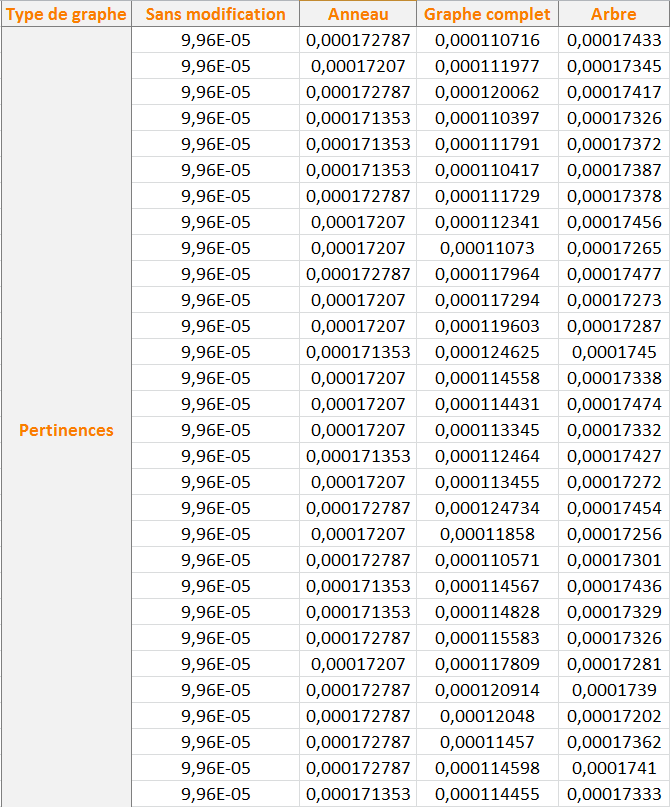
\includegraphics[scale = 0.5]{Captures/ranking2.PNG}\\
		La cible est de pertinence forte. \\
		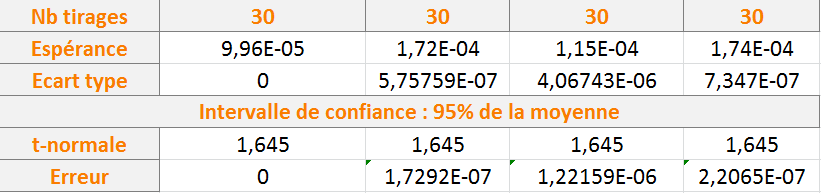
\includegraphics[scale = 0.5]{Captures/ranking3.PNG}\\
		En regardant les espérances on observe que c'est l'anneau est l'abre qui impactent le plus la pertinence de la cible.
		On observe aussi que les erreurs sont inférerieurs à 0,000015 on peut donc faire confiance aux résultats.\\
		Regardons les trois courbes en annexe.\\
		La courbe rouge représente la loi normale, la noire est la fonction de densité. 




	\subsection{Conclusion sur l'impact de chaque structure}


\section{III.	Expériences avec un graphe de degré aléatoire}
	Ici nous allons créer un graphe de 100 sommets de degré aléatoire. C'est à dire que chaque sommet sera relié au même nombre de sommets au sein du graphe.

	\subsection{Résultats des tests}
		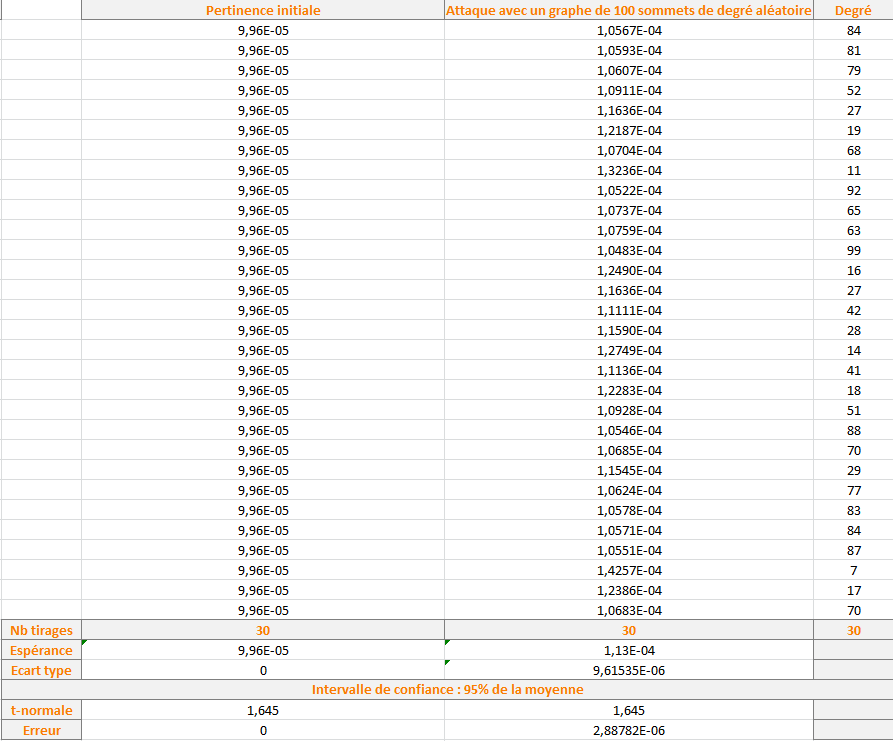
\includegraphics[scale = 0.5]{Captures/ranking4.PNG}\\
		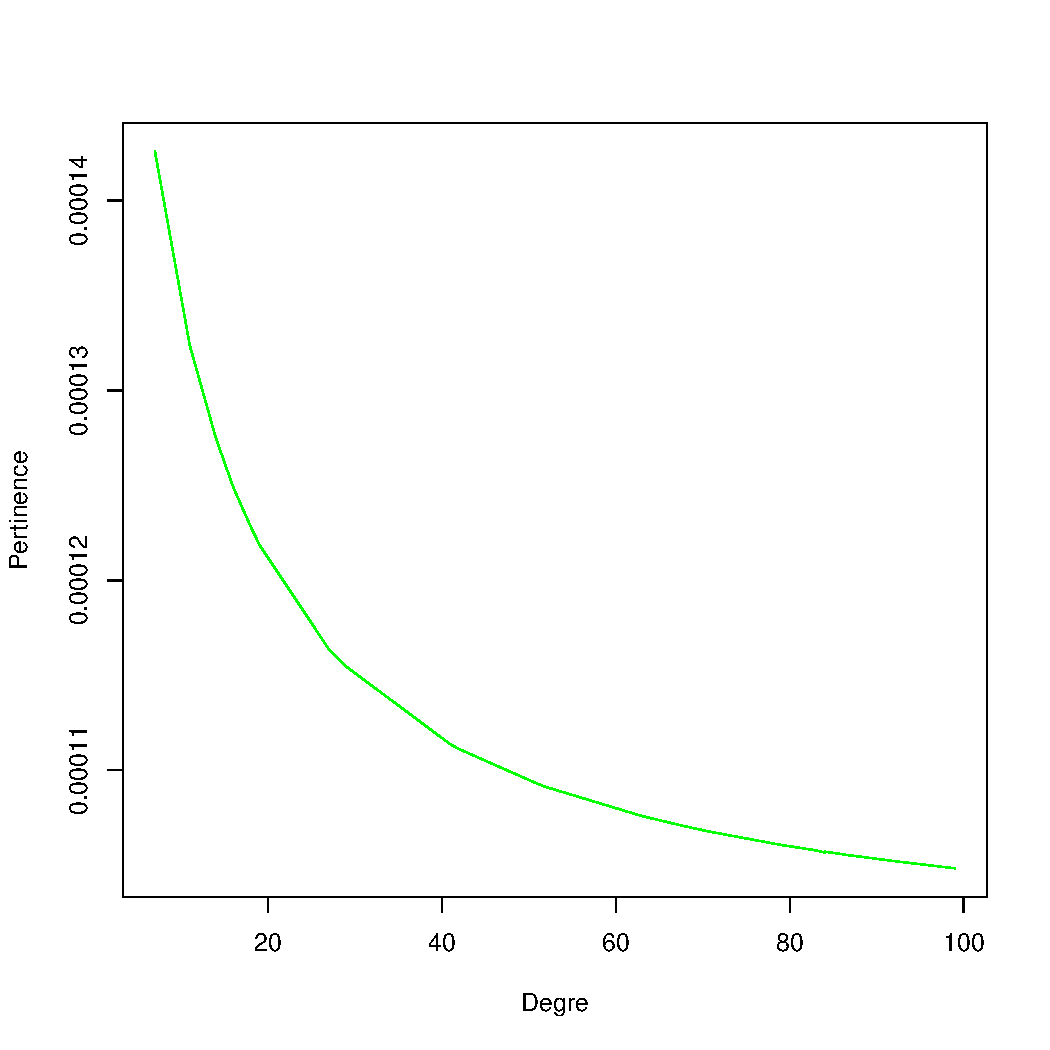
\includepdf{../R/Degre_aleatoire/degre.pdf}
	
	\subsection{Analyses}
		On observe que plus le degré est fort, moins la pertinence de la cible est modifié. Ici l'espérance de la pertinence de la cible apres attaque est de 1.13e-04, ce qui est 
		meilleur que la pertience de la cible lors des tests initiaux avec un graphe complet a 100 sommets (1.05e-04). Ainsi cette structure est plus eficace que le graphe complet.
		De plus cette structure a l'avantage d'etre moins detectable que l'anneau ou le graphe complet car le degré varie. En effet détecter un anneau ou un graphe complet est beaucoup plus aisé 
		que de détecter un graphe de degré X.
	
\section{IV.	Expériences sur l'efficacité}
	
	\subsection{Résultats des tests}
		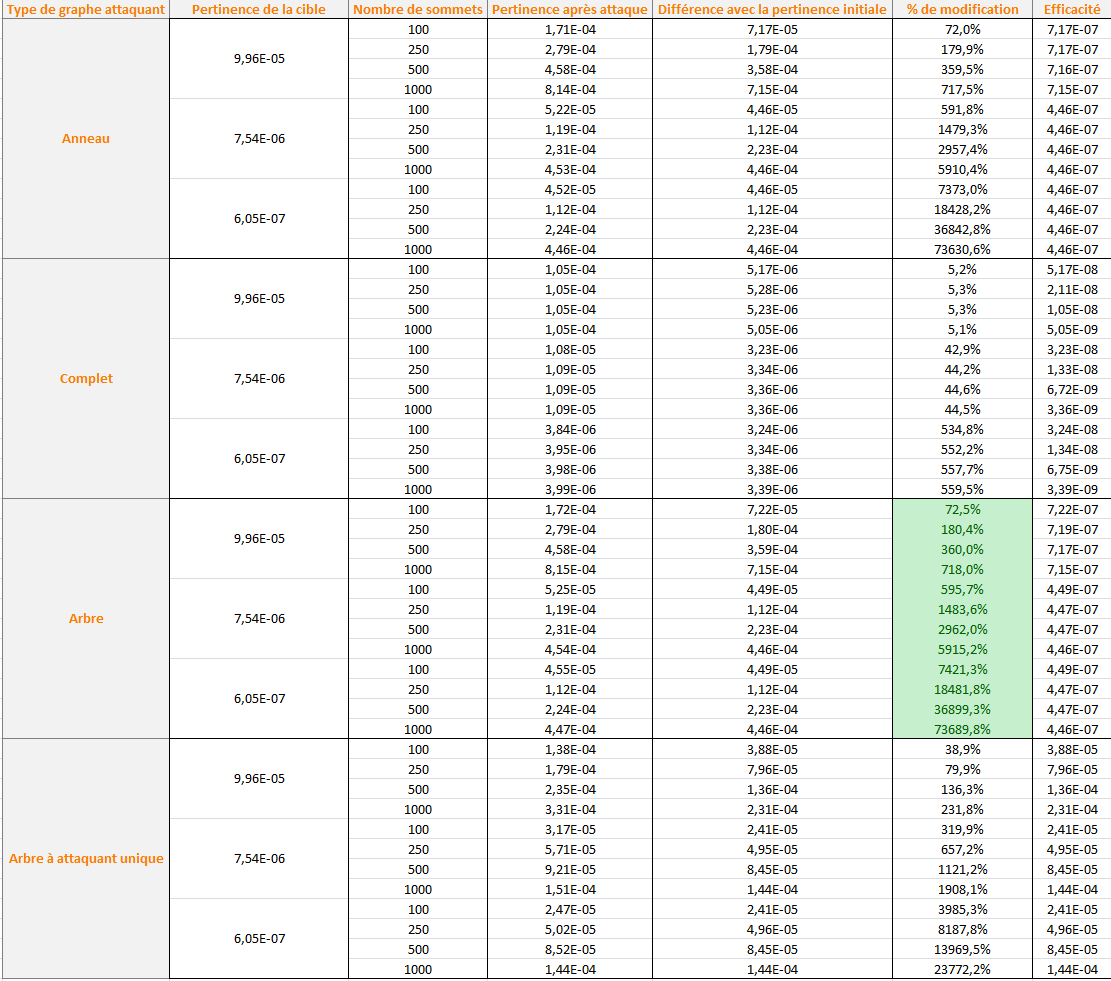
\includegraphics[scale = 0.5]{Captures/ranking5.PNG}\\
		Ici nous avons testé chaque structure sur trois cibles différentes, tout en faisant varier le nombre de sommets par structure. 
		Le pourcentage de modification est calculé ainsi que l'efficacité calculé en divisant la différence par rapport a la pertinence initiale par le nombre de sommets ajoutés.\\
	\subsection{Analyses}
		On observe que, toute pertinences confondus, la structure qui modifie le plus la cible est l'arbre, suivis de l'anneau, de l'arbre à attaquant unique et enfin du graphe complet.
		Cela confirme nos hypothèses des tests initiaux. La raison de cet efficacité est que la pertinence ne se disperse que tres peu dans ces structures, ce qui permet d'attaquer 
		la cible efficacement. Par exemple dans un anneau chaque sommet recoit la pertinence d'un de ses voisins puis pointe sur la cible. Ainsi la pertinence est équitablement répartie et peut dispersé au sein de la structure.
		Pour l'arbre on observe un phénomène similaire car chaque sommet est relié à son sommet père et à la cible. On peut expliquer la légère différence entre arbre et anneau par le fait 
		que plus on monte dans l'arbre, plus la pertinence est forte. Ainsi les attaques des sommets les plus haut dans l'arbre sont plus efficaces sur la cible.\\
		
		On observe que, pour toute structures confondus, la différence avec la pertinence initiale est quasiment identique entre une cible moyenne (7.54e-06) et faible (6.05e-07).
		C'est à dire que on modifie autant la cible qu'elle soit de pertinence moyenne ou faible. Ainsi on peut en conclure que les cibles en dessous de Xe-06 sont toutes trés similaires à attaquer.\\
		
		Pour l'anneau, le graphe complet et l'arbre on observe que la différence avec la pertinence initiale augmente de manière linéaire avec l'augmentation du nombre de sommets.
		par exemple pour l'arbre avec une cible forte on passe de 7.22e-5, 1.80e-4, 3.59e-4, 7.15e-4 pour 100, 250, 500 et 1000 sommets. Ce qui est presque parfaitement linéaire.
		Ce phénomène arrive quelquesoit la pertinence de la cible. Ainsi on peut en conclure que pour une attaque la plus efficace possible il faut augmenter le nombre de sommets au maximum.
		Cependant plus il y a de sommets, plus il est facile pour la cible de reconnaitre une attaque. Une stratégie raisonable serait d'utiliser un arbre de 500 sommets, 
		ce qui modifie la pertinence de la cible de 360\%, tout en ne représentant que 0.18\% du graphe du web. De plus une structure en arbre peut être difficile à reconnaitre si l'attaquant décide 
		de modifier légèrement sa structure. Par exemple enlever certains liens pointant vers la cible peuvent donner cela : 
		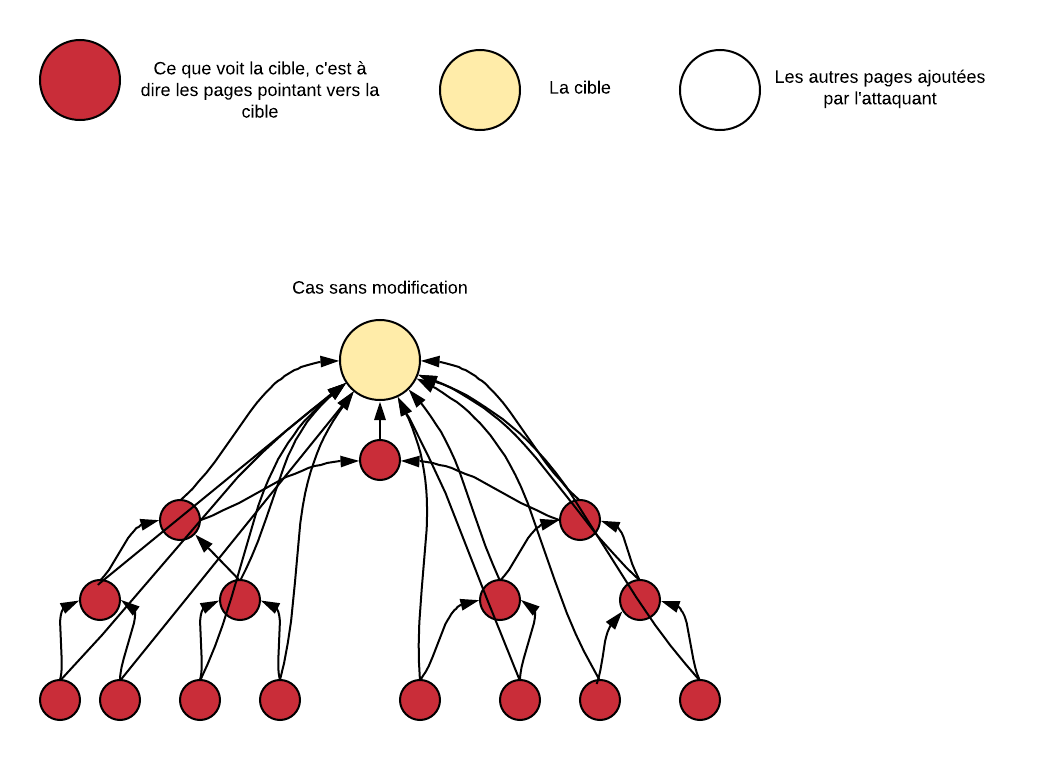
\includegraphics[scale = 0.5]{Captures/diagramme1.png}\\
		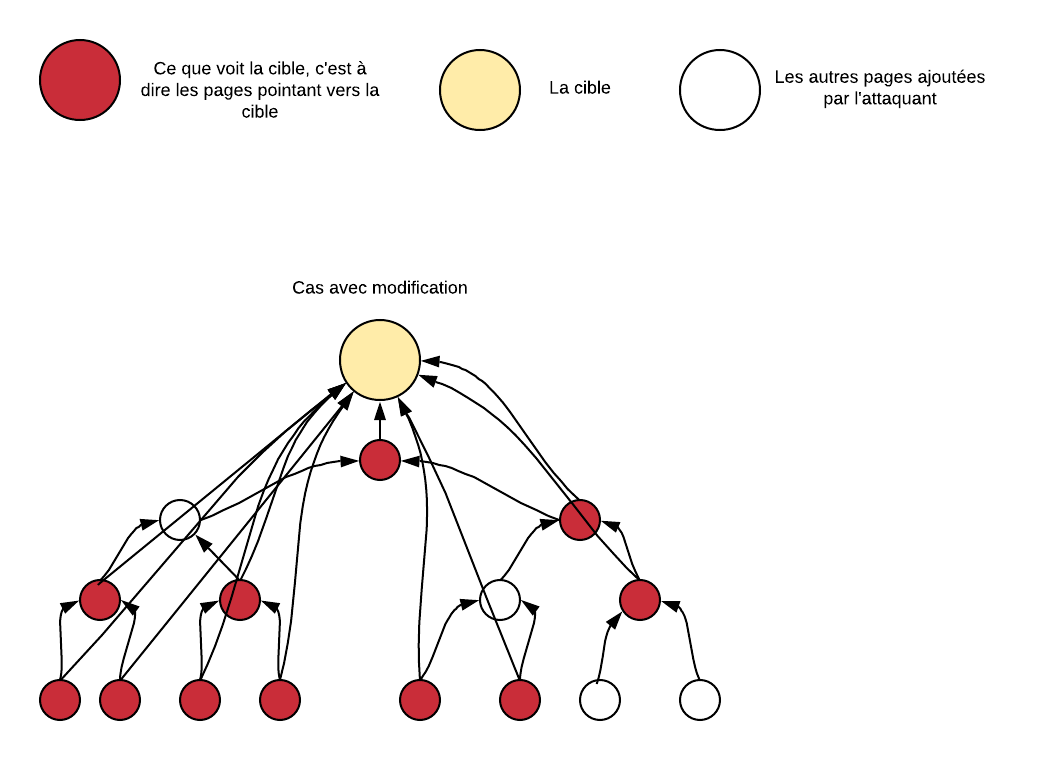
\includegraphics[scale = 0.5]{Captures/diagramme2.png}\\
		La cible ne peut voir que les pages qui pointe directement sur elle, c'est à dire les sommets en rouge.
		La seconde structure est légèrement moins efficace mais elle rend plus difficile la detection de l'arbre par la cible. En effet les sommets ne sont plus reliées ensemble en forme d'arbre du point de vu la cible.
		C'est donc une stratégie possible.\\
		
		On observe que les valeurs d'efficacité les plus grandes sont pour l'arbre a attaquant unique. Cela s'explique par le fait que un seul sommet est relié a la cible dans cette structure.
		Cependant les pourcentages de modifications sont bien plus faible que pour l'arbre ( 38\% contre 72\% pour une cible forte à 100 sommets attaquants).
		Mais cette structure reste très utile pour des cibles moyennes ou faible. Ainsi une startégie interessante pour les cibles faibles serait d'utiliser un arbre a attaquant unique.
		Son avanatge majeur est qu'il est tres difficile a détecter car un seul sommet est directement relié a la cible.\\
	
\section{Conclusions}

\section{Annexe}
		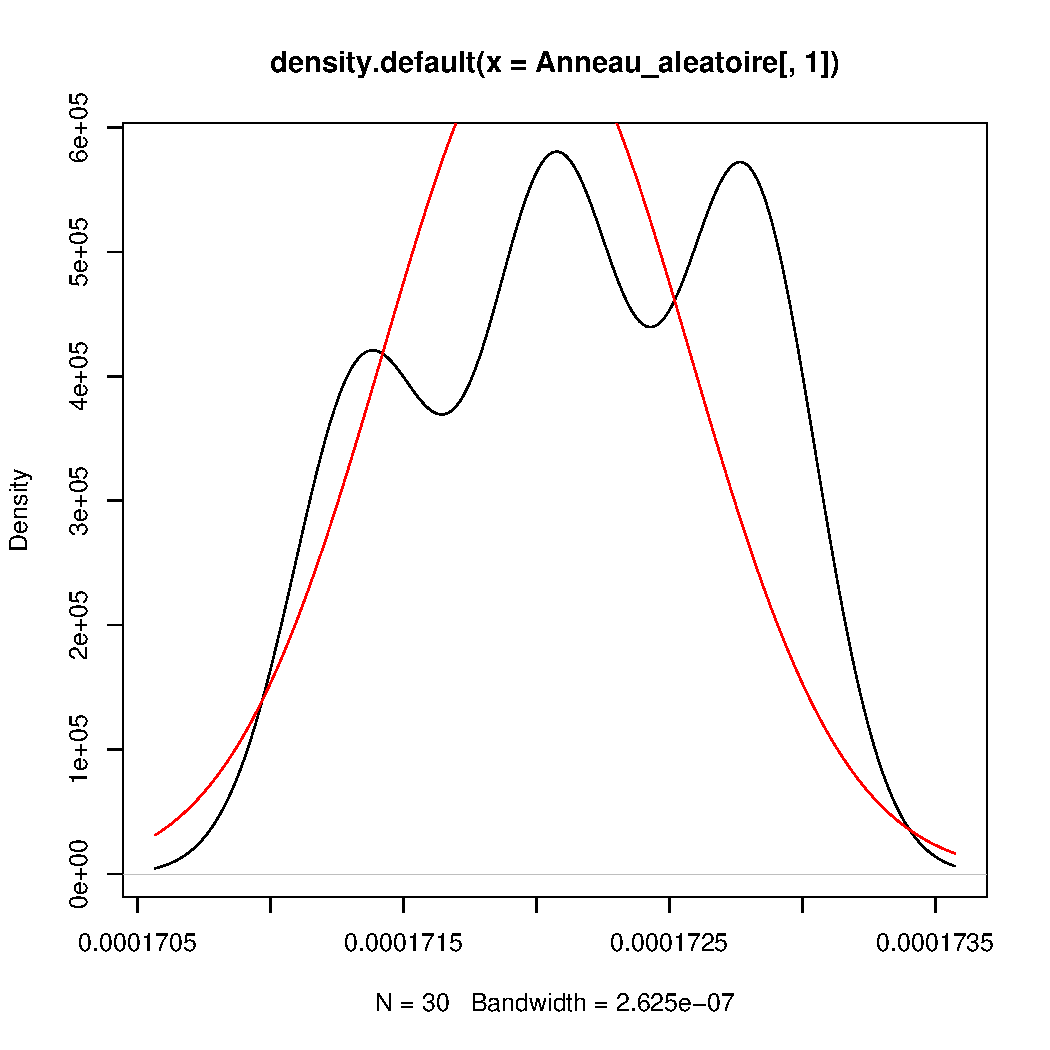
\includepdf{../R/Nombre_de_graphe_aleatoire/Anneau.pdf}
		
		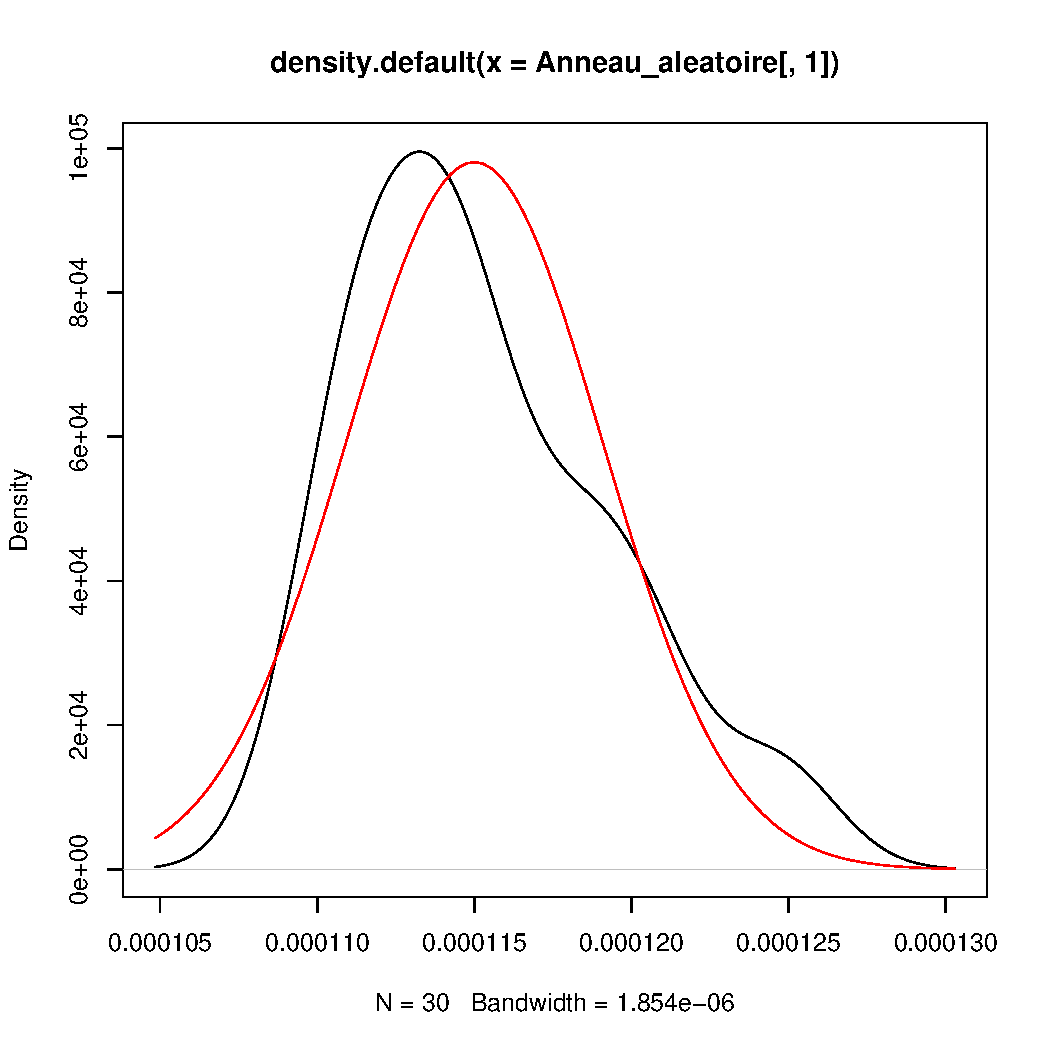
\includepdf{../R/Nombre_de_graphe_aleatoire/Complet.pdf}

		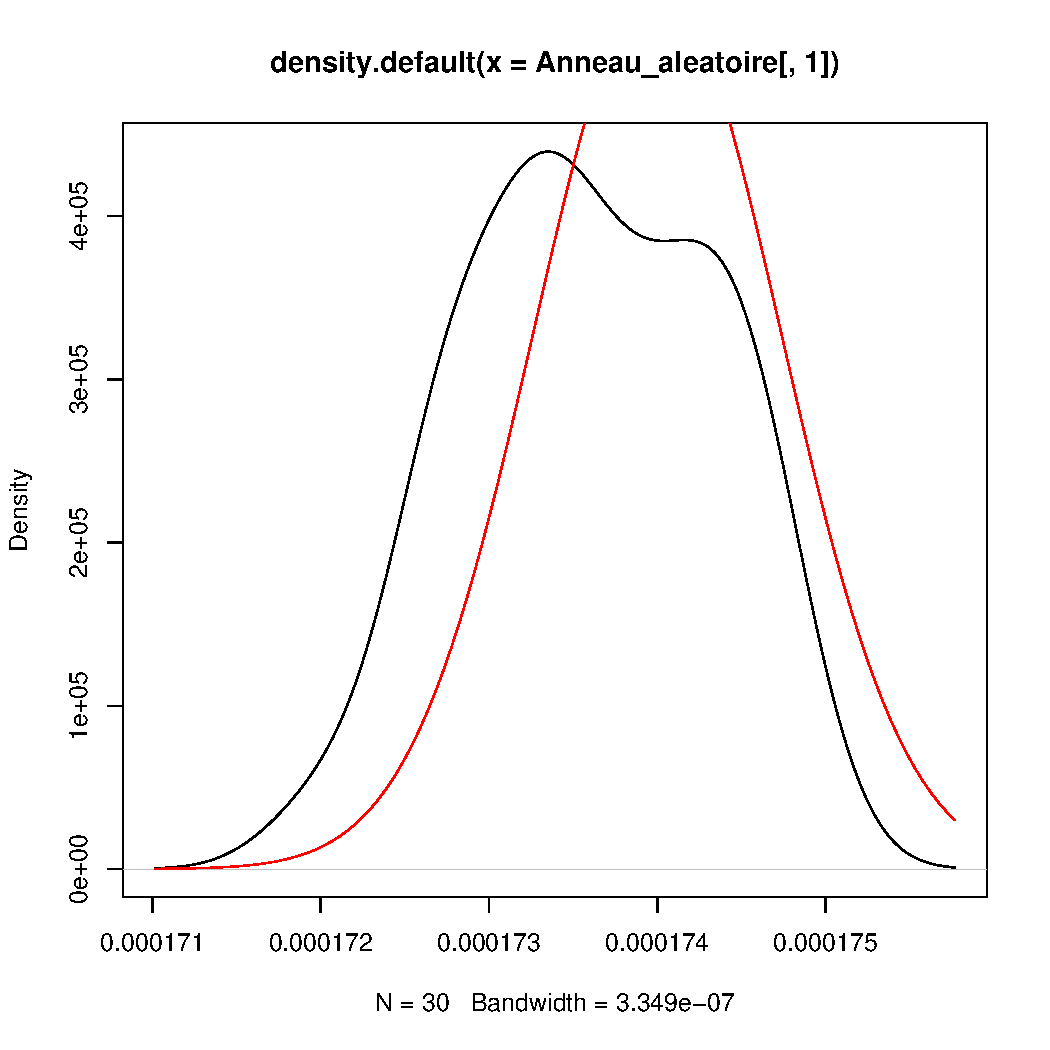
\includepdf{../R/Nombre_de_graphe_aleatoire/Arbre.pdf}

\end{document}
